\documentclass[12pt,letterpaper]{article}

%%%% Packages %%%%%%%%%%%%%%%%%%%%%%%%%%%%%%%%%%%%%%%%%%%%%%%%%%%%%%%%%%%%%%%%%%
\usepackage{graphicx} % Required for inserting images

% Links
\usepackage{hyperref}

% Page format
\usepackage[letterpaper, margin=1in]{geometry}

% References package
\usepackage[style=authoryear,sorting=anyt]{biblatex}
\addbibresource{references.bib}

% Dates
\usepackage[USenglish]{babel}
\usepackage[nodayofweek,level]{datetime}
\newcommand{\mydate}{\formatdate{4}{4}{2024}}

% Appendix
\usepackage[toc,page]{appendix}

% Code section
\usepackage{listings}
\usepackage{color}
\definecolor{dkgreen}{rgb}{0,0.6,0}
\definecolor{gray}{rgb}{0.5,0.5,0.5}
\definecolor{mauve}{rgb}{0.58,0,0.82}
\lstset{frame=tb,
  language=Bash,
  aboveskip=3mm,
  belowskip=3mm,
  showstringspaces=false,
  columns=flexible,
  basicstyle={\small\ttfamily},
  numbers=none,
  numberstyle=\tiny\color{gray},
  keywordstyle=\color{blue},
  commentstyle=\color{dkgreen},
  stringstyle=\color{mauve},
  breaklines=true,
  breakatwhitespace=true,
  tabsize=3
}

% float for position
\usepackage{float}

% subfigures
\usepackage{subcaption}
\usepackage[font=small,labelfont=bf]{caption}
%%%% Packages %%%%%%%%%%%%%%%%%%%%%%%%%%%%%%%%%%%%%%%%%%%%%%%%%%%%%%%%%%%%%%%%%%

\begin{document}

\begin{center}
% Title
{\LARGE \bfseries Exploring the Effects of Plasma Treatment on \textit{Sorghum bicolor}: \par
An RNA-Seq Analysis\par}
\vspace{0.5cm}

% Author Name
{\Large \textbf{Fangyi Li}\par}
\vspace{0.5cm}

% Student Number
{\small Student Number: 1005937774\par}
\vspace{0.5cm}

% Course Code
{\small Course: BCB430Y 2023-2024\par
Advanced Special Project in Bioinformatics and Computational Biology\par}
\vspace{0.5cm}

% Supervisors
{\small \textbf{Advisory Team:}\par
Professor Nicholas J. Provart\par
Professor Takamasa Okumura\par
Professor Eiji Nambara\par
Vincent Lau, MSc.\par}
\vspace{0.5cm}

% Date
\selectlanguage{USenglish}
{\small \mydate} % This will print the current date in the format "September 10, 2023"
% If you need a specific date format or a static date, replace with your preferred format
\vspace{0.5cm}
    
\end{center}

\begin{abstract}
    Plasma treatment, encompassing various technologies such as cold plasma and atmospheric plasma, holds promise in agricultural research for enhancing plant growth, improving crop productivity, and alleviating environmental stresses. Despite its potential, the molecular mechanisms governing the response of plants to plasma treatment, especially in crops like \textit{Sorghum bicolor}, remain poorly understood. In this study, we utilized RNA sequencing (RNA-Seq) analysis coupled with bioinformatics tools to explore the transcriptional response of \textit{Sorghum bicolor} to plasma treatment. Our differential gene expression analysis unveiled significant alterations in gene expression profiles across different conditions, with a notable number of genes showing up and down-regulation in response to plasma treatment compared to untreated (wild-type) plants. Functional enrichment analysis, employing established databases or tools such as agriGO, g:Profiler, and PlantRegMap, elucidated the biological processes, molecular functions, and cellular components associated with the differentially expressed genes. Noteworthy enrichments included processes related to photosynthesis, response to environmental stimuli, and metabolic pathways. Moreover, visualization of gene expression patterns using the Sorghum eFP Browser provided insights into the spatial and temporal dynamics of gene expression changes induced by plasma treatment. Overall, our findings deepen the understanding of the molecular mechanisms underlying \textit{Sorghum bicolor}'s response to plasma treatment, with potential implications for enhancing crop productivity and sustainability in agricultural practices.
    
    \vspace{0.5cm}
    \textbf{Keywords}: \textit{Sorghum bicolor}, Plasma Treatment, RNA-Seq, eFP Browser
\end{abstract}

% Start a new page after abstract
\clearpage


\section{Introduction}
\textit{Sorghum bicolor}, commonly known as sorghum, stands out as a vital cereal crop globally, prized for its versatility and resilience across diverse agroecological landscapes. Its capacity to thrive under various climatic conditions and its multifaceted utility in food, feed, fodder, and bioenergy production underscore its pivotal role in bolstering global food security and advancing agricultural sustainability \parencite{mccormick2018sorghum}.

Plasma treatment, an emerging technology in agricultural research, has garnered increasing attention for its potential to bolster plant growth, enhance crop productivity, and mitigate biotic and abiotic stresses. Functioning as the fourth state of matter, plasma comprises a highly reactive ionized gas housing an array of reactive oxygen and nitrogen species, ultraviolet radiation, and electromagnetic fields. When applied to plants, plasma treatment induces physiological and biochemical transformations at the molecular level, triggering shifts in gene expression patterns and activating defense mechanisms that fortify plant resilience against environmental stressors \parencite{attriplasma}.

However, despite the burgeoning interest in plasma treatment as a sustainable agricultural modality, the molecular intricacies underlying the plant's response to plasma treatment still need to be more adequately understood, particularly in crops like sorghum. Understanding how plasma treatment influences gene expression patterns in sorghum holds promise for shedding light on the molecular underpinnings of plasma-induced stress tolerance and growth promotion, thus offering potential avenues for enhancing crop productivity and sustainability.

In this study, we employed RNA sequencing (RNA-Seq) analysis in conjunction with bioinformatics tools to probe the transcriptional response of \textit{Sorghum bicolor} to plasma treatment. By characterizing differential gene expression patterns, functional enrichment analyses, and gene expression visualization, we aimed to elucidate the molecular mechanisms governing the plant's response to plasma treatment and pinpoint potential candidate genes associated with plasma-induced stress tolerance and growth promotion in sorghum.

\section{Methods}

\subsection{Experimental Design}

\begin{table}[H]
\centering
\begin{tabular}{|l|l|c|}
\hline
\textbf{Condition}                  & \textbf{Label Name} & \textbf{Number of Replicates} \\ \hline
Dry Seed                            & Seed Dry            & 3                             \\ \hline
Imbibed Seed (no plasma treatment)  & Seed WT             & 3                             \\ \hline
Imbibed Seed with Plasma Treatment  & Seed Plasma         & 3                             \\ \hline
Shoot from Imbibed Seed             & Shoot WT            & 3                             \\ \hline
Shoot from Imbibed Seed with Plasma & Shoot Plasma        & 3                             \\ \hline
\end{tabular}
\caption{Overview of Experimental Conditions and Replicates.}
\end{table}

\subsubsection{Dry Seed Condition}
RNA-Seq data for the dry seed condition were obtained from a previous study titled "Gene expression analysis of \textit{Sorghum bicolor} BTx623 \parencite{federhen2012ncbi}." These reads represented the initial gene expression state before undergoing any experimental treatment, providing a comparable condition for comparative analyses with seeds subjected to imbibition and other treatments.

\subsubsection{Imbibed Seed Conditions}
Seeds were subjected to controlled imbibition conditions to simulate natural germination processes. Each condition involved the incubation of ten seeds per bed, with the bed comprising paper pulp (1.2 g) mixed with water (2.7 mL) in polymer dishes. The incubation environment was maintained under a 16-hour light cycle with a photosynthetic photon flux density (PPFD) of 100 $\mu$mol m\textsuperscript{-2} s\textsuperscript{-1} and a temperature of 28°C. Seeds in specific conditions were treated with plasma during imbibition, with the "1-day imbibed seed with plasma treatment" condition aimed at investigating any potential effects of plasma treatment on gene expression compared to seeds without plasma treatment. Sampling was conducted one day after seed imbibition, with RNA-Seq data collected from three seeds per condition, replicated three times for two conditions. This baseline data represented the gene expression profile at the onset of seed imbibition.

\subsubsection{Shoot Conditions}
Following seed imbibition, seeds were replanted into pods to facilitate shoot growth. Each pod accommodated one seed and was filled with a soil mixture comprising culture soil (Sakata Super Mix, Sakata Seed Co., Tokyo, Japan) and vermiculite at a ratio of 2:1. Nutrient supplementation was provided by adding 1000-fold diluted HYPONEX 3L to the soil of 6L. Pod growth conditions included a 16-hour light cycle with a PPFD of 80 $\mu$mol m\textsuperscript{-2} s\textsuperscript{-1} and a temperature of 28°C. It is important to note that shoots were not subjected to plasma treatment directly. Instead, shoots were grown from seeds that had undergone either plasma or no treatment. Sampling of shoot tissues was performed four weeks after seed imbibition. RNA-Seq data were collected from one individual per condition and replicated three times for two conditions. This baseline data represented the gene expression profile of shoots grown from seeds subjected to the imbibition process, with and without plasma treatment.


\subsection{Bioinformatics Analysis}

\subsubsection{Read Alignment with HISAT2}
The raw sequencing reads obtained from the experimental design section underwent alignment using HISAT2 (Hierarchical Indexing for Spliced Alignment of Transcripts 2). HISAT2 was selected for its fast and sensitive alignment capabilities. It is specifically designed for aligning RNA-Seq reads to reference genomes while accounting for known splice junctions \parencite{kim2019hisat2}.

\clearpage

\begin{lstlisting}[caption={Example Bash Code for Read Alignment with HISAT2 and Samtools.},captionpos=b]
#!/bin/bash

# Loading modules needed
module load hisat2
module load samtools

# 1. Convert GTF to HISAT2's known-splice-site format
hisat2_extract_splice_sites.py Sbicolor_annotations.gtf > splice_sites.txt
hisat2_extract_exons.py Sbicolor_annotations.gtf > exons.txt

# 2. Build the HISAT2 index
hisat2-build -p 8 --ss splice_sites.txt --exon exons.txt Sbicolor_reference.fa Sbicolor_index

# 3. Align RNA-Seq reads using HISAT2 (paired-end)
hisat2 -p 8 --phred33 -x Sbicolor_index -1 read_1.fq -2 read_2.fq -S sample.sam 

# 4. Convert SAM to BAM and sort
samtools view -@ 8 -b -o sample_unsorted.bam sample.sam
samtools sort -@ 8 -o sample.bam sample_unsorted.bam
\end{lstlisting}

The alignment process began with indexing the reference genome using HISAT2. For this study, the genome annotation file in GTF (Gene Transfer Format) and the genome reference file in FASTA format were obtained and converted from Phytozome \parencite{goodstein2012phytozome}. This step involved generating an index of the reference genome to facilitate rapid alignment.

Once the reference genome was indexed, the sequencing reads in FASTQ format were aligned to the indexed reference genome using HISAT2. HISAT2 employs a two-step approach to identify potential splice junctions and align reads accordingly during alignment.

The alignment process output was a file in SAM (Sequence Alignment/Map) format containing information about the alignment of each read to the reference genome. Subsequently, the SAM files were converted into sorted BAM (Binary Alignment/Map) files using Samtools \parencite{samtools}. Sorted BAM files are advantageous for downstream analyses due to their compressed format and indexed alignment positions.


\subsubsection{Read Counting with featureCounts}
Following the alignment of sequencing reads to the reference genome, the subsequent step in the RNA-Seq analysis pipeline involved quantifying the number of reads aligned to each genomic feature, such as genes or transcripts. This quantification was conducted using featureCounts, a widely utilized software tool for read counting in RNA-Seq analysis known for its accuracy and efficiency \parencite{liao2014featurecounts}.

\clearpage

\begin{lstlisting}[caption={Example R code for Read Counting with featureCounts.},captionpos=b]
# Run featureCounts
fc_result <- Rsubread::featureCounts(files = list.files(path = bam_path, pattern = "\\.bam$", full.names = TRUE), 
                                        annot.ext = gtf,
                                        isGTFAnnotationFile = TRUE,
                                        GTF.featureType = "exon",
                                        GTF.attrType = "gene_id",
                                        useMetaFeatures = TRUE,
                                        isPairedEnd = TRUE)
  
# Extract raw counts
counts <- fc_result$counts
\end{lstlisting}

FeatureCounts takes the aligned reads in BAM format as input and a genome annotation file in GTF format. In this study, the genome annotation file in GTF format was obtained from Phytozome. It furnishes vital information about the genomic coordinates of genes and other genomic features essential for accurate read counting.

The featureCounts process began with input preparation, where aligned reads in BAM format, and the genome annotation file in GTF format were provided as input to featureCounts. Subsequently, featureCounts assigned each aligned read to genomic features based on their alignment positions, handling reads that overlapped with multiple features or fell within ambiguous regions according to specified parameters.

The output of featureCounts was a count matrix, where each row represented a genomic feature (e.g., gene), and each column represented a sample. This count matrix was the foundation for downstream analyses, such as differential gene expression analysis using tools like DESeq2.


\subsubsection{Differential Gene Expression Analysis with DESeq2}
Following read counting with featureCounts, the count matrix containing the read counts for each genomic feature across samples underwent differential gene expression analysis using DESeq2. DESeq2, a widely used R/Bioconductor package, is designed explicitly for analyzing RNA-Seq data, particularly for identifying genes that are differentially expressed between conditions \parencite{deseq2}.

\begin{lstlisting}[caption={Example R Code for Differential Gene Expression Analysis with DESeq2.},captionpos=b]
# Perform DESeq2 analysis
dds <- DESeq2::DESeqDataSetFromMatrix(counts, colData, design = ~ condition)
dds <- DESeq2::DESeq(dds)

# Get Results
res <- DESeq2::results(dds)
\end{lstlisting}

The DESeq2 analysis began with the import of the count matrix generated by featureCounts into R using the DESeq2 package. Upon import, DESeq2 normalized the count data to correct for differences in library size and composition across samples, ensuring that gene expression levels were comparable.

Subsequently, DESeq2 utilized a negative binomial distribution to model read counts and employed a generalized linear model framework to identify differentially expressed genes. The model accounted for variability in sequencing depth and biological variability between replicates. Statistical testing was then conducted to determine whether the expression of each gene was significantly different between conditions.

Genes with adjusted p-values below a specified threshold (e.g., FDR \textless 0.05) were considered statistically significant. DESeq2 output included lists of differentially expressed genes, corresponding fold changes and statistical significance values. These results provided insights into the up-regulated or down-regulated genes under different experimental conditions.


\subsubsection{Functional Analysis Tools}

Functional analysis tools are essential for interpreting the biological significance of differentially expressed genes identified through RNA-Seq analysis. These tools allow researchers to explore the functional roles and biological processes associated with the identified genes.

This study utilized several functional analysis tools to gain insights into the biological functions, pathways, and regulatory networks associated with the differentially expressed genes. The functional analysis tools employed include:

\begin{enumerate}
\item \textbf{agriGO}: agriGO is a web-based tool specifically designed for Gene Ontology (GO) enrichment analysis in agricultural species. It enables the identification of overrepresented GO terms among a list of genes of interest, providing insights into the biological processes, molecular functions, and cellular components associated with the genes \parencite{tian2017agrigo}.

\item \textbf{g:Profiler}: A versatile tool for functional enrichment analysis of gene lists. It integrates multiple databases, including GO, KEGG, and Reactome pathways, to identify enriched functional categories and pathways, offering comprehensive annotations and visualizations for interpreting gene lists \parencite{reimand2007gProfiler}.

\item \textbf{PlantRegMap}: A comprehensive database of plant transcriptional regulatory networks and regulatory elements. It provides insights into transcription factors, target genes, and regulatory interactions in various plant species, aiding in exploring regulatory networks associated with differentially expressed genes \parencite{tian2020plantregmap}.
\end{enumerate}


\subsubsection{eFP Browser}
The eFP (electronic Fluorescent Pictograph) browser is a valuable tool for visualizing gene expression data \parencite{winter2007electronic}. In our study, we utilized TPM (Transcripts Per Million) values calculated with the eFP browser to visualize gene expression patterns of interest \parencite{wagner2012tpm}. This visualization allowed researchers to observe spatial and temporal gene expression patterns across various tissues and developmental stages.

TPM values were calculated using the formula:
\[TPM=\frac{n_{g}}{N\cdot l_{g}}(10^3)(10^6)\] where $n_{g}$ is the number of reads/fragments for the gene, $N$ is the sum of reads/fragments, and $l_{g}$ is the length of the gene \parencite{wagner2012tpm}.

Moreover, correlation analysis was conducted between TPM values of dry seed samples and those from previous databases. This comparative analysis provided valuable insights by aligning current gene expression profiles with established data from prior studies. By leveraging the eFP browser for visualization and conducting correlation analysis, researchers better understood gene expression dynamics in plant growth, development, and environmental responses.

\section{Results}

\subsection{Differential Gene Expression Analysis}

\subsubsection{DESeq2 Results} 

\begin{figure}[H]
\begin{subfigure}{\textwidth}
    \centering
    \frame{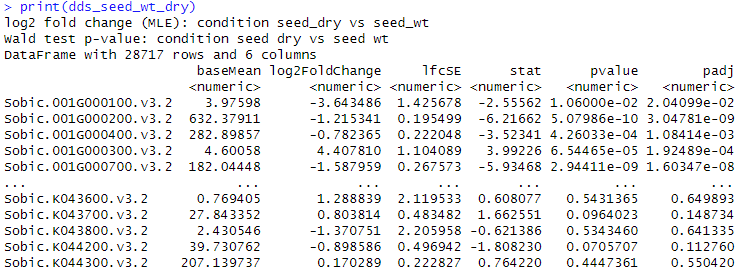
\includegraphics[width=.9\linewidth]{figures/dds_seed_wt_dry.png}}
    \caption{Seed WT vs. Dry}
    \label{fig:enter-label}
\end{subfigure}\par
\begin{subfigure}{\textwidth}
    \centering
    \frame{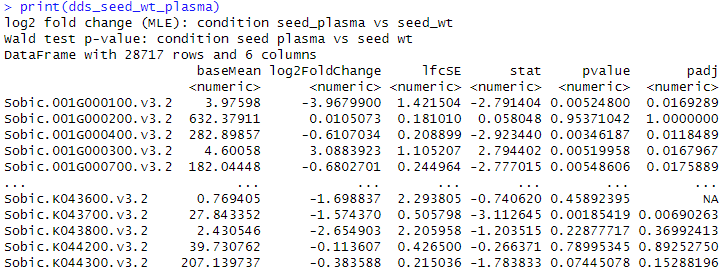
\includegraphics[width=.9\linewidth]{figures/dds_seed_wt_plasma.png}}
    \caption{Seed WT vs. Plasma}
    \label{fig:enter-label}
\end{subfigure}\par
\begin{subfigure}{\textwidth}
    \centering
    \frame{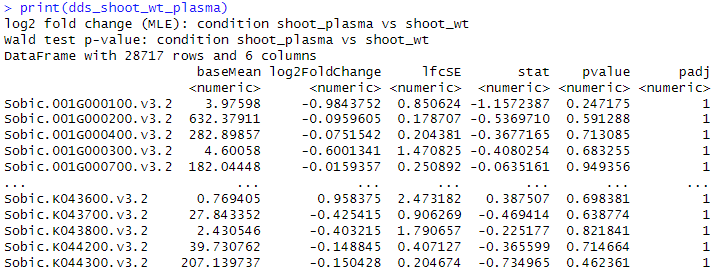
\includegraphics[width=.9\linewidth]{figures/dds_shoot_wt_plasma.png}}
    \caption{Shoot WT vs. Plasma}
    \label{fig:enter-label}
\end{subfigure}
\caption{DESeq2 Results of (a) Seed WT vs. Dry, (b) Seed WT vs. Plasma, and (c) Shoot WT vs. Plasma Comparisons.}
\end{figure}

Figure 1 presents result tables for each comparison, containing key parameters such as the mean of normalized counts for all samples (baseMean), log2 fold change (log2FoldChange), standard error (lfcSE), Wald statistic (stat), Wald test p-value (pvalue), and Benjamini-Hochberg adjusted p-value (padj). The DESeq2 analysis utilized an adjusted p-value threshold of \textless 0.05. Differentially expressed genes were identified based on a log2 fold change threshold of \textgreater 1 for up-regulated and \textless -1 for down-regulated genes. These results unveiled significant transcriptomic changes across different experimental conditions, indicating the dynamic nature of gene regulation in the studied organism \parencite{deseq2}.

\begin{table}[H]
\centering
\begin{tabular}{|l|c|c|}
\hline
\multicolumn{1}{|c|}{\textbf{Comparison}} & \textbf{Up-regulated Genes} & \textbf{Down-regulated Genes} \\ \hline
Seed WT vs. Dry                           & 4737                                  & 6852                                    \\ \hline
Seed WT vs. Plasma                        & 1976                                  & 3603                                    \\ \hline
Shoot WT vs. Plasma                       & 0                                     & 0                                       \\ \hline
\end{tabular}
\caption{Number of Up and Down-regulated Genes for Each Comparison.}
\end{table}

Table 2 summarizes the number of up and down-regulated genes identified for each comparison, highlighting the magnitude of gene expression alterations in response to various experimental treatments.

\subsubsection{PCA Plot}
Principal Component Analysis (PCA) was utilized to visualize the overall patterns of variation in gene expression across samples. The PCA plot reveals distinct clustering patterns among the samples based on their transcriptional profiles \parencite{pearson1901pca}.

\begin{figure}[H]
\begin{subfigure}[b]{0.5\textwidth}
    \centering
    \frame{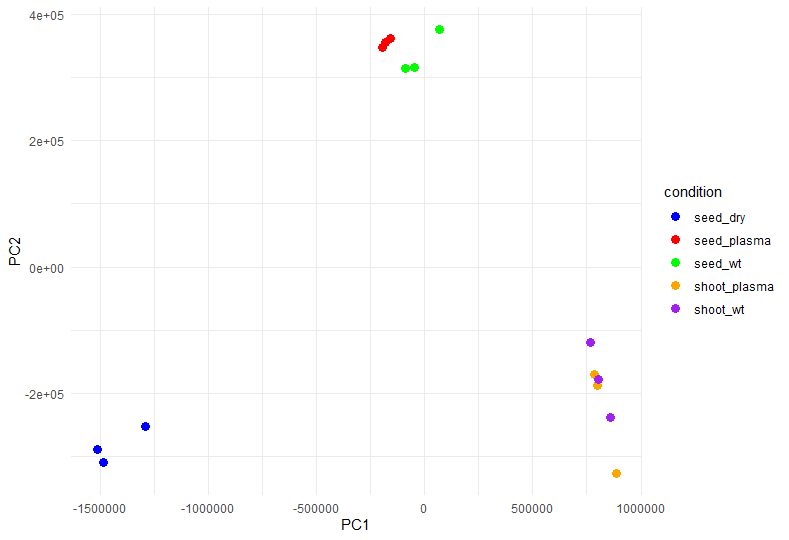
\includegraphics[width=\textwidth]{figures/pca_2d.png}}
    \caption{2D PCA}
    \label{fig:enter-label}
\end{subfigure}
\begin{subfigure}[b]{0.5\textwidth}
    \centering
    \frame{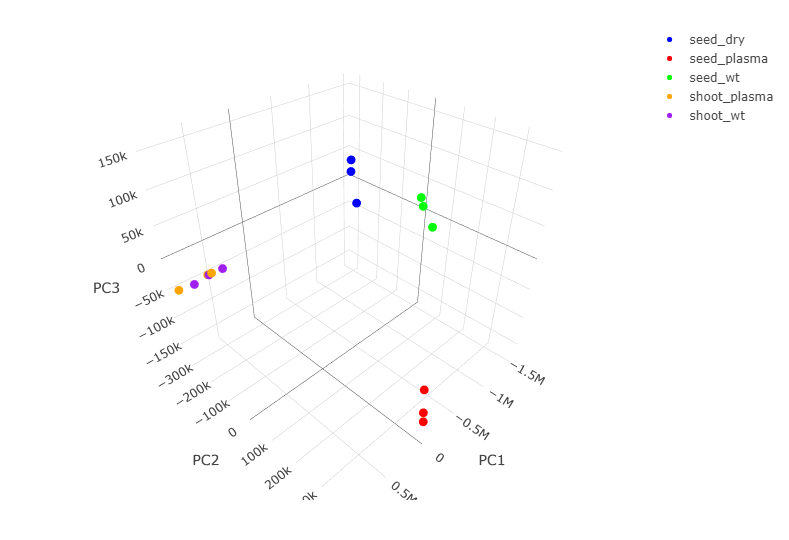
\includegraphics[width=\textwidth]{figures/pca_3d.png}}
    \caption{3D PCA}
    \label{fig:enter-label}
\end{subfigure}
\caption{PCA Plots in (a) 2D and (b) 3D.}
\end{figure}

Figure 2 illustrates that replicates of Seed Dry, Seed WT, and Seed Plasma samples form three distinct clusters, indicating similar gene expression profiles within each experimental condition. Conversely, replicates of Shoot WT and Shoot Plasma samples cluster together as a single group, suggesting similar gene expression profiles between these conditions.

The observed clustering patterns in the PCA plot provide valuable insights into the relationships between samples and highlight the transcriptional differences between the experimental conditions.

\subsubsection{MA Plot}
MA plots were utilized to visualize gene expression differences between conditions. Each point on the plot represents a gene, with the x-axis indicating the average expression level (A) and the y-axis showing the log-fold change (M) in gene expression between conditions.

\begin{figure}[H]
\centering
\begin{subfigure}[b]{0.32\textwidth}
    \centering
    \frame{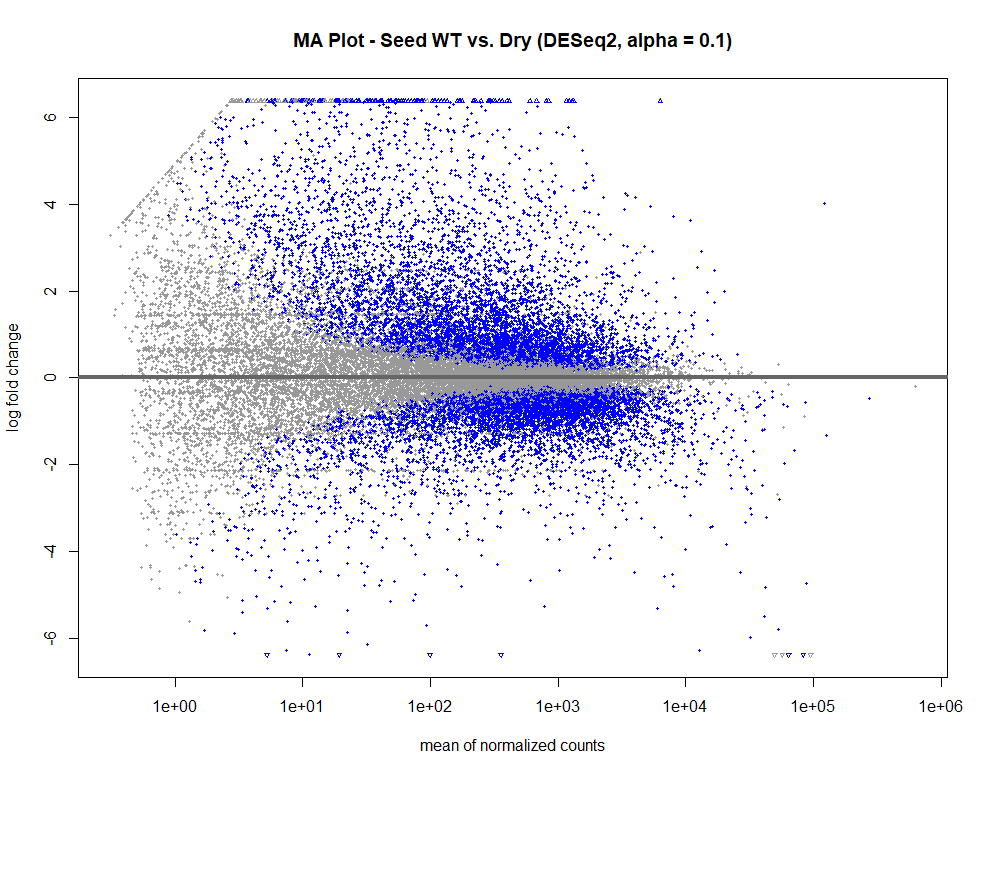
\includegraphics[width=\textwidth]{figures/MA_DESeq2_seed_wt_dry.png}}
    \caption{Seed WT vs. Dry}
    \label{fig:enter-label}
\end{subfigure}
\begin{subfigure}[b]{0.32\textwidth}
    \centering
    \frame{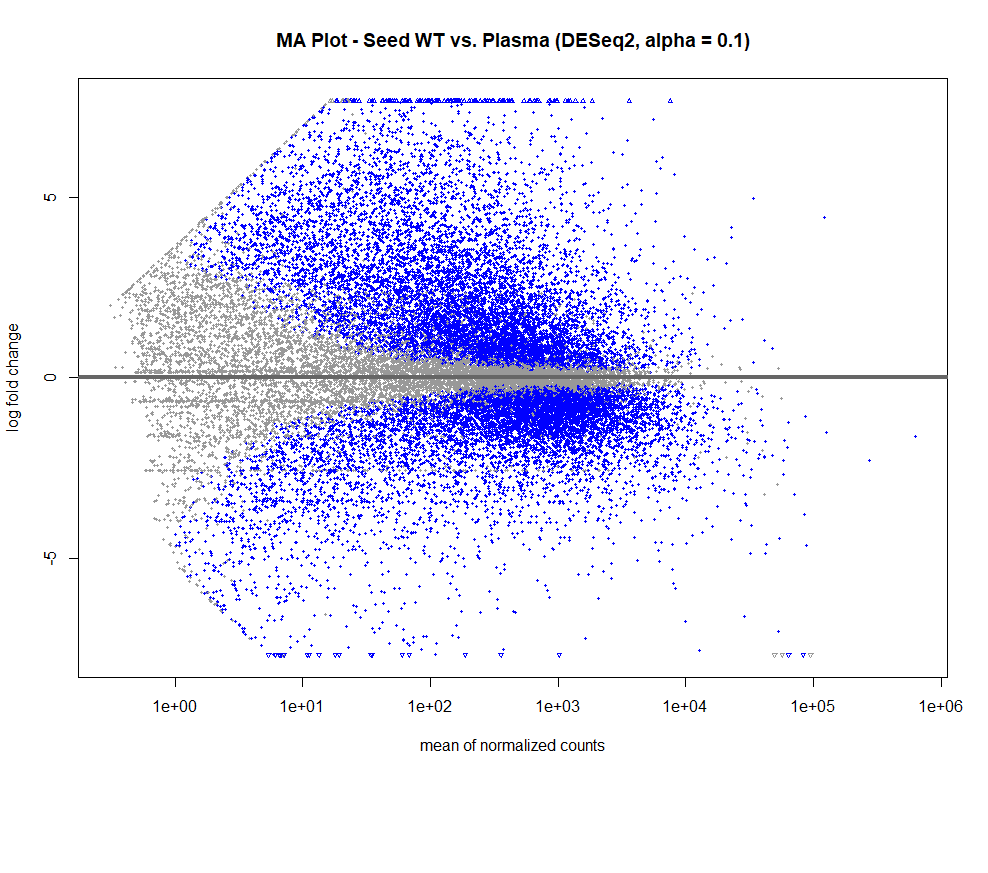
\includegraphics[width=\textwidth]{figures/MA_DESeq2_seed_wt_plasma.png}}
    \caption{Seed WT vs. Plasma}
    \label{fig:enter-label}
\end{subfigure}
\begin{subfigure}[b]{0.32\textwidth}
    \centering
    \frame{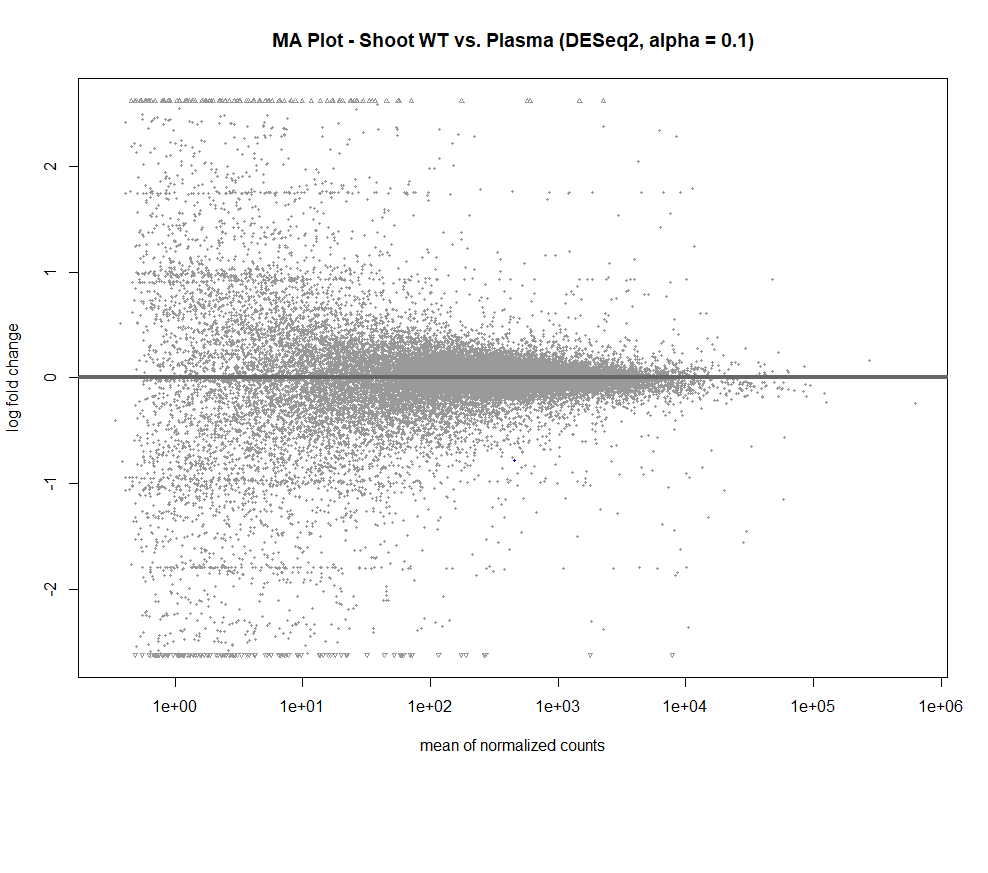
\includegraphics[width=\textwidth]{figures/MA_DESeq2_shoot_wt_plasma.png}}
    \caption{Shoot WT vs. Plasma}
    \label{fig:enter-label}
\end{subfigure}
\caption{MA Plots of (a) Seed WT vs. Dry, (b) Seed WT vs. Plasma, and (c) Shoot WT vs. Plasma Comparisons.}
\end{figure}

In Figure 3, comparing (a) Seed WT vs. Dry and (b) Seed WT vs. Plasma, two distinct sets of points are observed: grey and blue. Grey points represent genes that do not meet the criteria for differential expression, while blue points highlight genes that are significantly differentially expressed (adjusted p-value \textless0.05 and log2 fold change \textgreater 1 or \textless -1). Notably, only the comparisons of (a) Seed WT vs. Dry, as well as (b) Seed WT vs. Plasma, exhibit blue points, indicating significant changes in gene expression between these conditions.

Blue points in these MA plots suggest that certain genes undergo significant changes in expression levels during seed imbibition and in response to plasma treatment. These findings provide valuable insights into the transcriptional dynamics associated with these experimental conditions.

\subsubsection{Volcano Plot}
Volcano plots were employed to visualize the relationship between statistical significance and fold change of gene expression between two conditions. In these plots, each point represents a gene, with the x-axis indicating the log2 fold change and the y-axis representing the statistical significance, typically measured as the adjusted p-value.

Three distinct sets of points are observed in the volcano plots: black, blue, and red. Black points represent genes that do not meet the criteria for differential expression. Blue points indicate genes with an adjusted p-value \textless 0.05, while red points highlight genes that not only have an adjusted p-value \textless 0.05 but also have a log2 fold change \textgreater 1 or \textless -1.

\begin{figure}[H]
\centering
\begin{subfigure}[b]{0.32\textwidth}
    \centering
    \frame{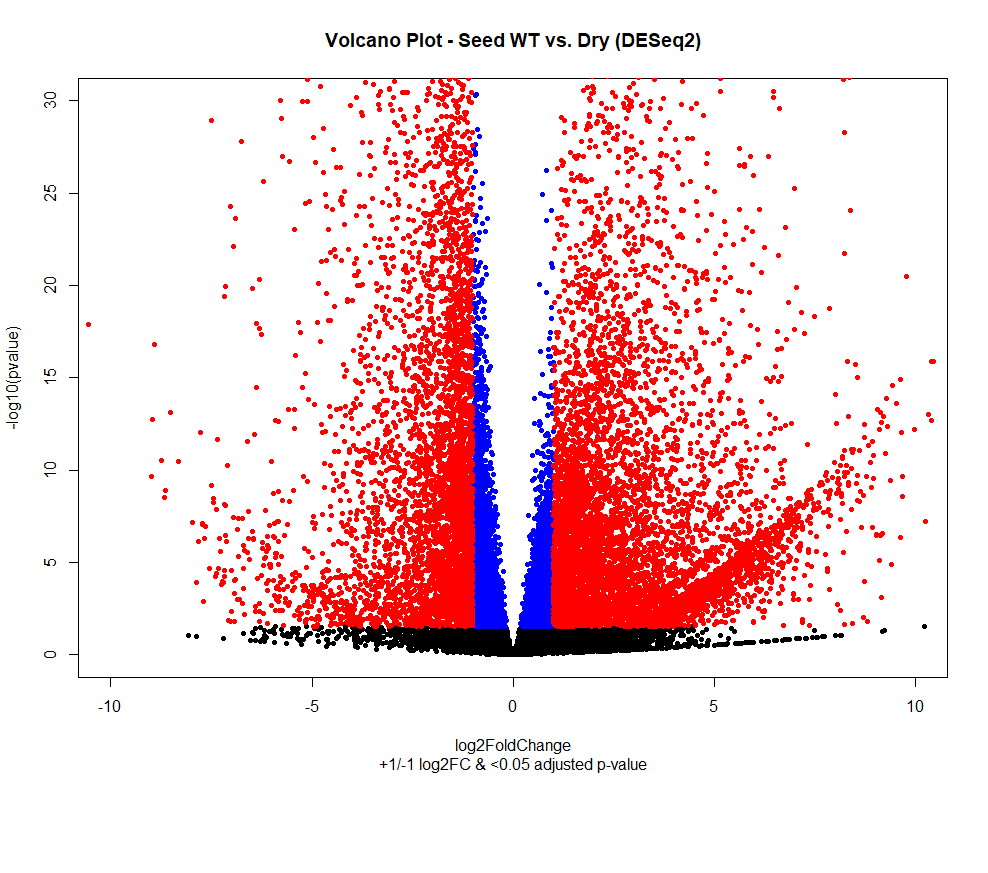
\includegraphics[width=\textwidth]{figures/Volcano_DESeq2_seed_wt_dry.png}}
    \caption{Seed WT vs. Dry}
    \label{fig:enter-label}
\end{subfigure}
\begin{subfigure}[b]{0.32\textwidth}
    \centering
    \frame{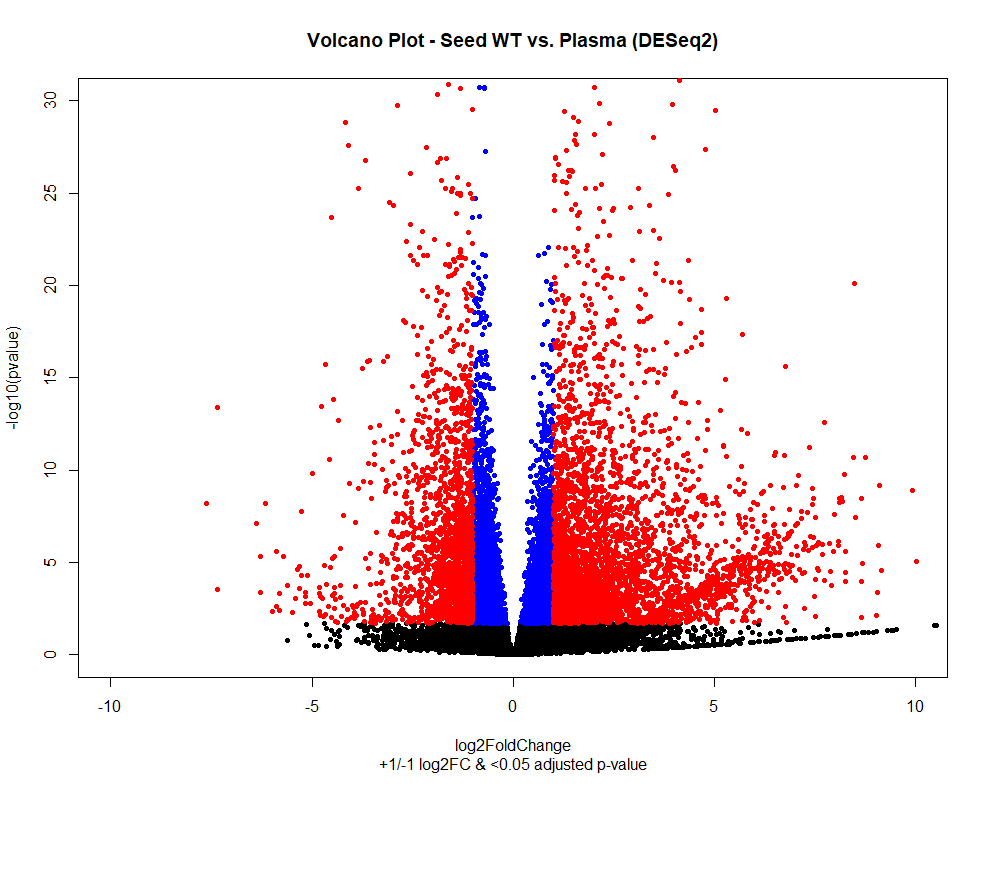
\includegraphics[width=\textwidth]{figures/Volcano_DESeq2_seed_wt_plasma.png}}
    \caption{Seed WT vs. Plasma}
    \label{fig:enter-label}
\end{subfigure}
\begin{subfigure}[b]{0.32\textwidth}
    \centering
    \frame{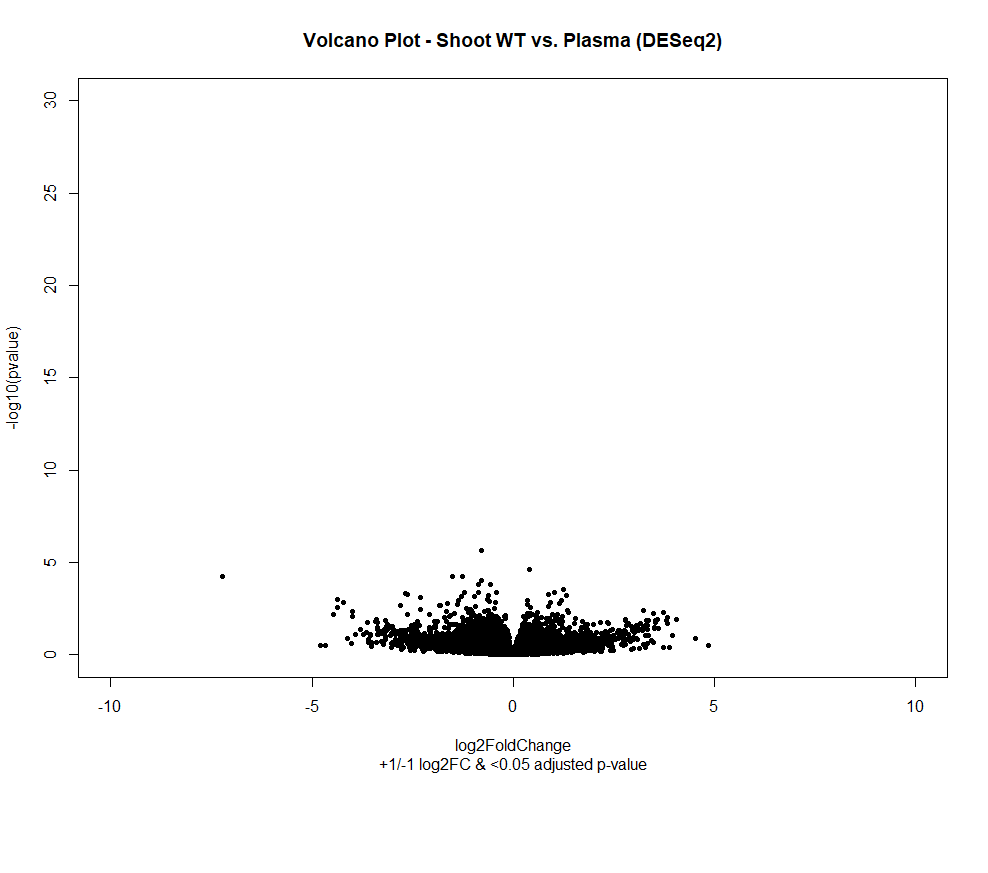
\includegraphics[width=\textwidth]{figures/Volcano_DESeq2_shoot_wt_plasma.png}}
    \caption{Shoot WT vs. Plasma}
    \label{fig:enter-label}
\end{subfigure}
\caption{Volcano Plots of (a) Seed WT vs. Dry, (b) Seed WT vs. Plasma, and (c) Shoot WT vs. Plasma Comparisons.}
\end{figure}

Figure 4 compares (a) Seed WT vs. Dry and (b) Seed WT vs. Plasma, exhibiting both blue and red points, indicating significant changes in gene expression between these conditions. In contrast, Figure 4 comparing (c) Shoot WT vs. Plasma only contains black points, indicating no significant differential gene expression between these conditions.

The presence of blue and red points in the volcano plots highlights genes with significant changes in expression levels, providing valuable insights into the transcriptional responses associated with seed imbibition and plasma treatment.

\subsection{Functional Analysis}
Functional analysis tools were utilized to uncover the biological processes and pathways influenced by gene expression changes in response to plasma treatment. The analysis concentrated on data comparing Seed WT and Seed Plasma conditions, as no differentially expressed genes were identified in the Shoot WT vs. Plasma comparison.

\subsubsection{agriGO}
\begin{figure}[H]
\begin{subfigure}[b]{1\textwidth}
    \centering
    \frame{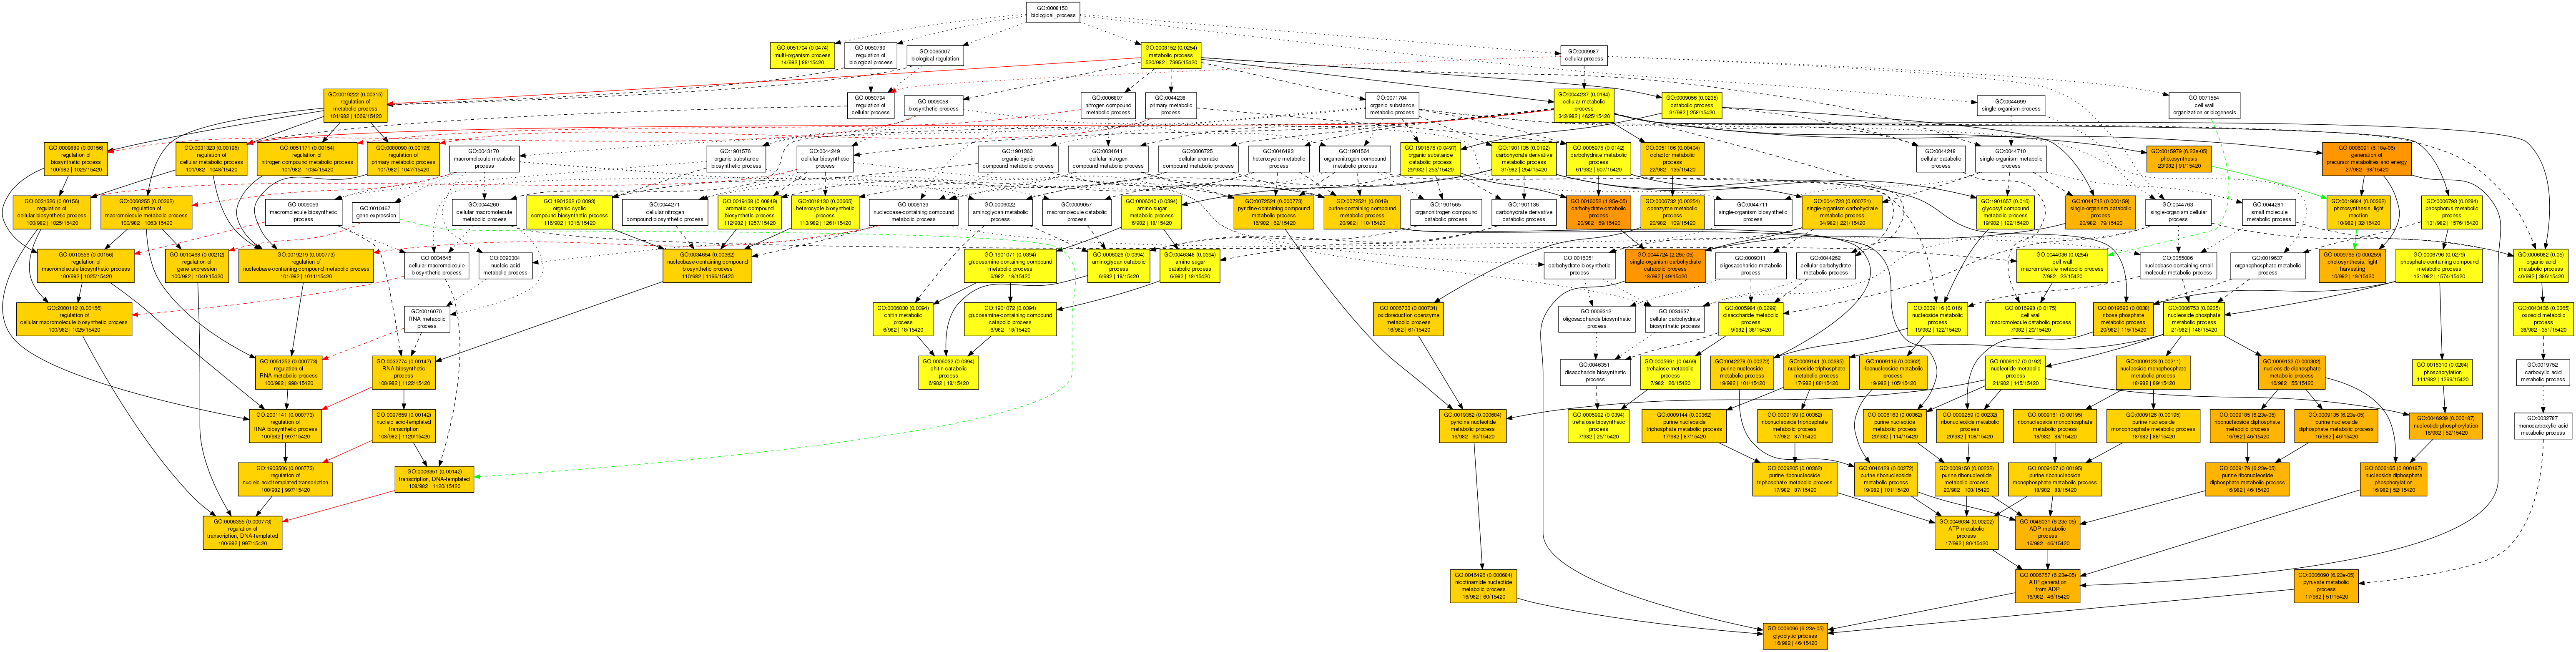
\includegraphics[width=\textwidth]{figures/agriGO_seed_wt_plasma_up_BP.png}}
    \caption{Up-regulated BP Ontology}
    \label{fig:enter-label}
\end{subfigure}\par
\begin{subfigure}[b]{1\textwidth}
    \centering
    \frame{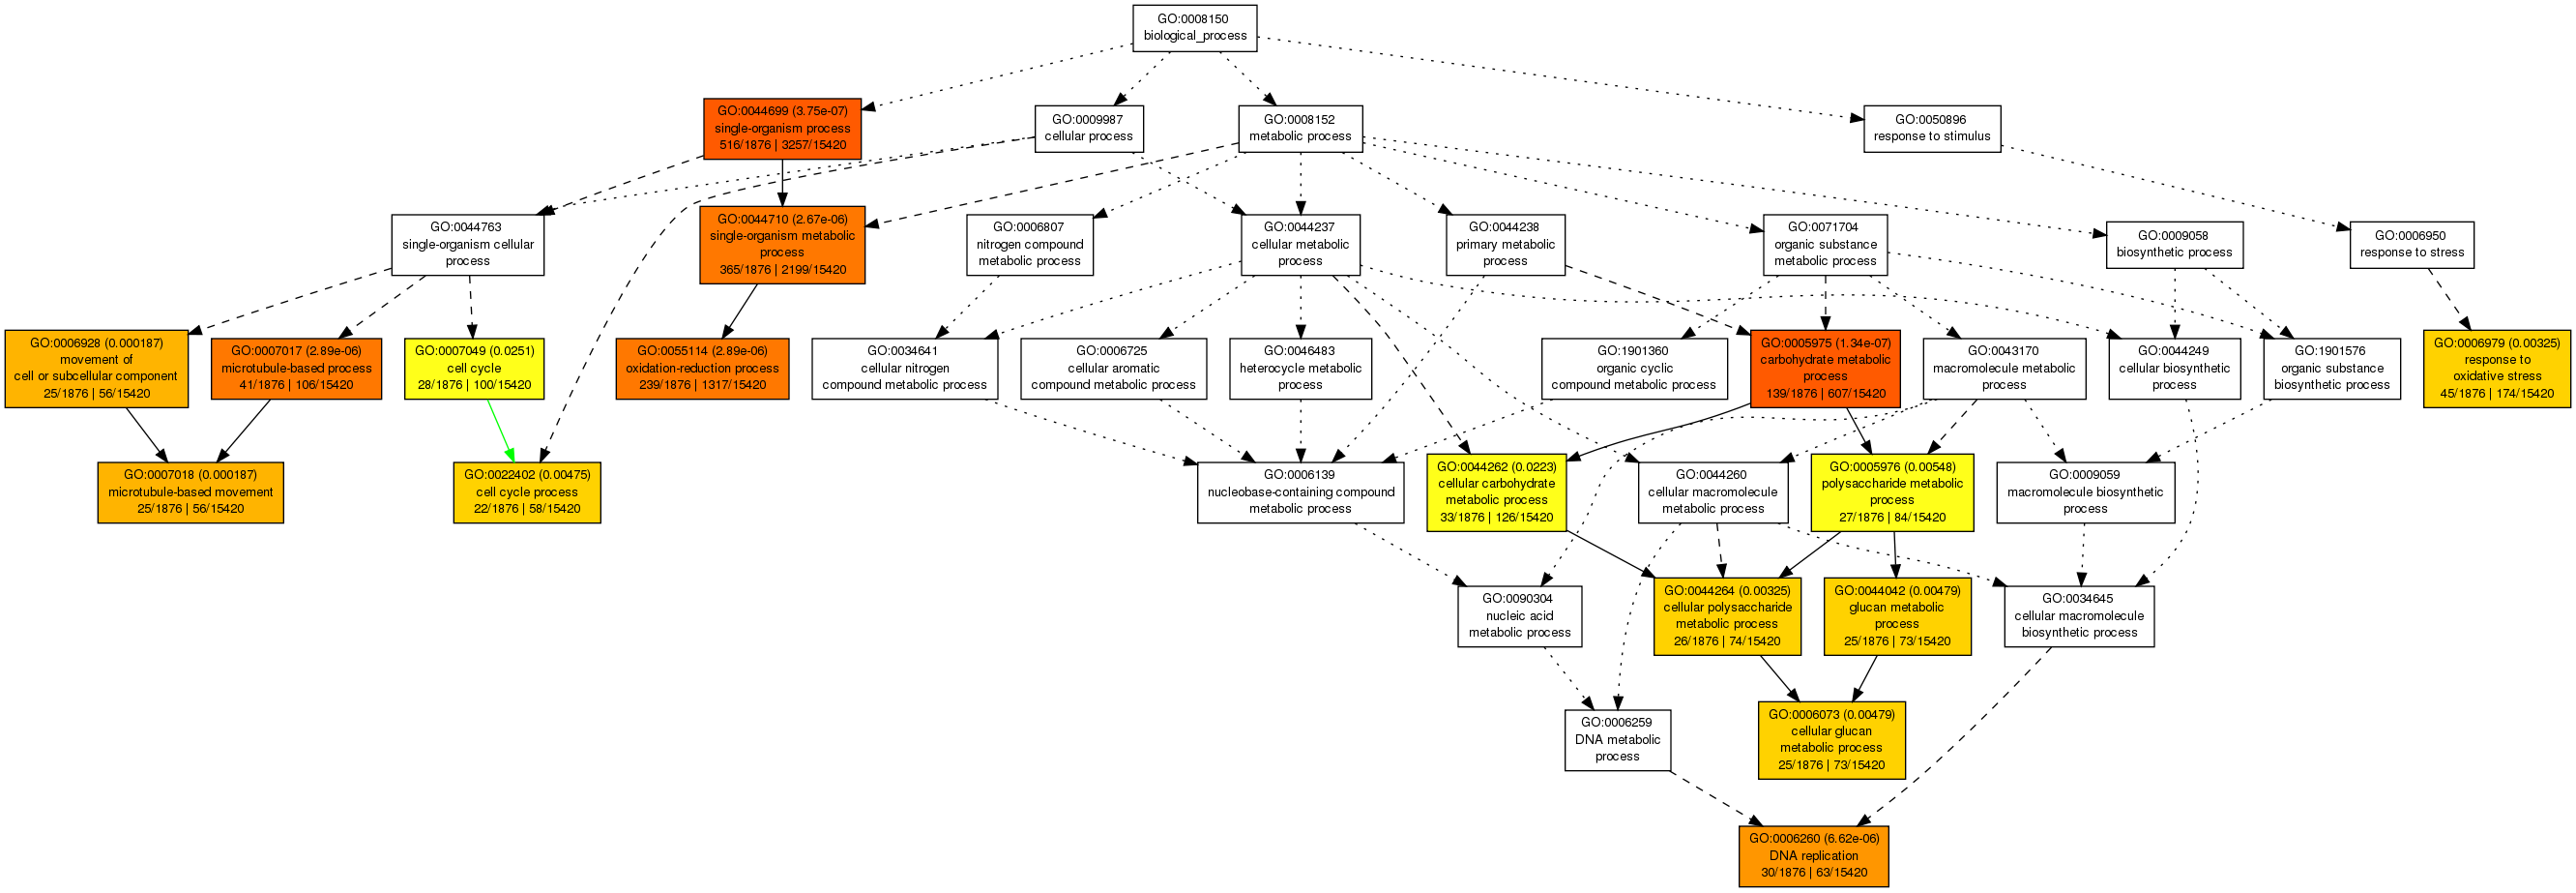
\includegraphics[width=\textwidth]{figures/agriGO_seed_wt_plasma_down_BP.png}}
    \caption{Down-regulated BP Ontology}
    \label{fig:enter-label}
\end{subfigure}
\caption{agriGO Biological Process Ontology of (a) Up-regulated and (b) Down-regulated Genes.}
\end{figure}

Figure 5 illustrates the functional analysis results conducted using agriGO, focusing on the biological processes associated with differentially expressed genes between Seed WT and Seed Plasma conditions \parencite{tian2017agrigo}.

Subfigure (a) displays the biological process graph of up-regulated genes, highlighting key GO terms related to metabolic processes and energy generation. Notable terms include "generation of precursor metabolites and energy," "carbohydrate catabolic process," and "photosynthesis," indicating enrichment of pathways involved in energy metabolism and carbohydrate utilization in response to plasma treatment.

Conversely, Subfigure (b) presents the biological process graph of down-regulated genes, revealing GO terms associated with diverse cellular processes such as carbohydrate metabolism, oxidation-reduction processes, and DNA replication. These findings suggest suppressing metabolic and cellular activities in response to plasma treatment, potentially reflecting adaptive responses to altered environmental conditions.

\begin{figure}[H]
    \centering
\begin{subfigure}[b]{0.4\textwidth}
    \centering
    \frame{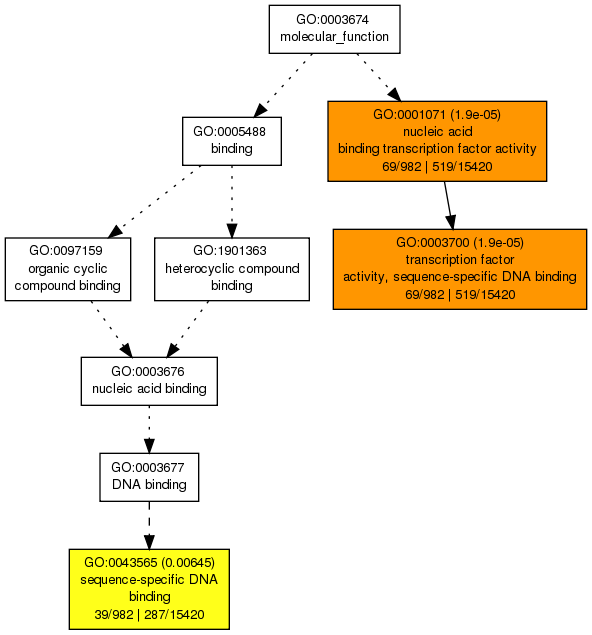
\includegraphics[width=\textwidth]{figures/agriGO_seed_wt_plasma_up_MF.png}}
    \caption{Up-regulated MF Ontology}
    \label{fig:enter-label}
\end{subfigure}
\begin{subfigure}[b]{0.55\textwidth}
    \centering
    \frame{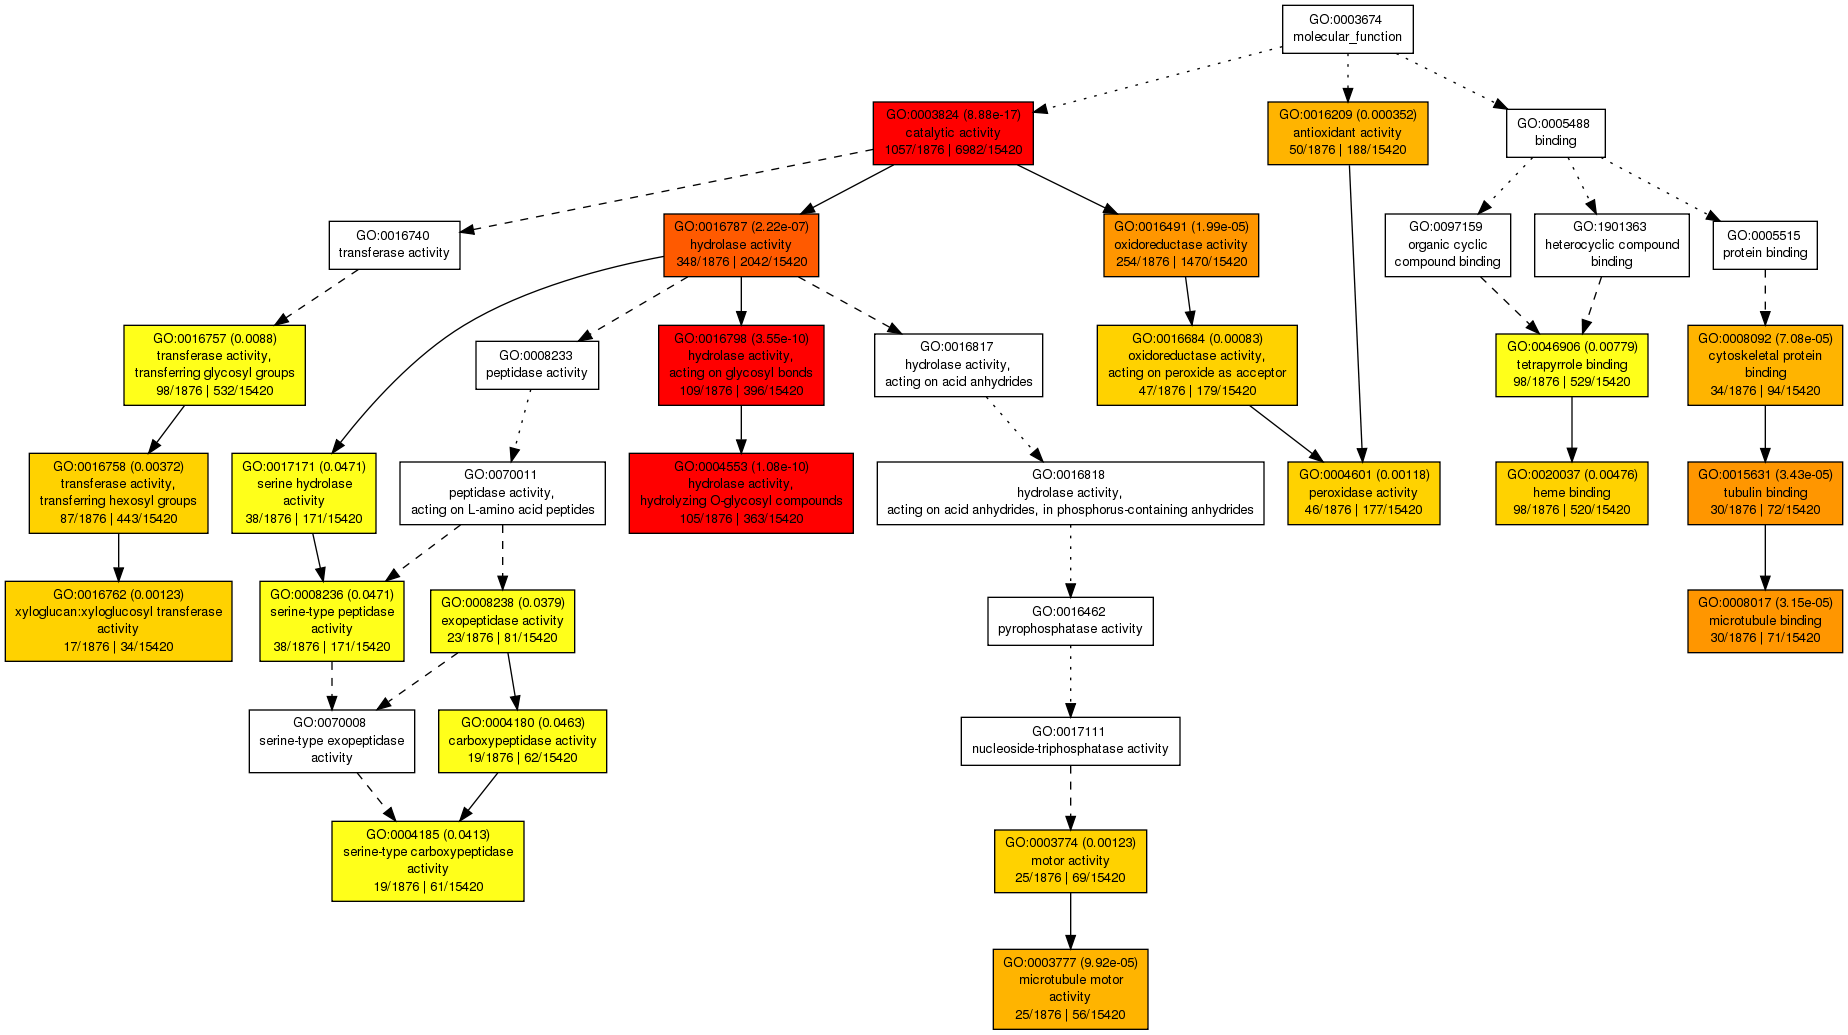
\includegraphics[width=\textwidth]{figures/agriGO_seed_wt_plasma_down_MF.png}}
    \caption{Down-regulated MF Ontology}
    \label{fig:enter-label}
\end{subfigure}
\caption{agriGO Molecular Function of Ontology (a) Up-regulated and (b) Down-regulated Genes.}
\end{figure}

Figure 6 provides insights into the molecular functions associated with differentially expressed genes between Seed WT and Seed Plasma conditions, as revealed by agriGO analysis \parencite{tian2017agrigo}.

Subfigure (a) illustrates the molecular function graph of up-regulated genes, highlighting key GO terms related to transcriptional regulation and enzymatic activities. Notable terms include "transcription factor activity," "sequence-specific DNA binding," and "carbohydrate kinase activity," suggesting an enrichment of regulatory and metabolic functions in response to plasma treatment.

Conversely, Subfigure (b) depicts the molecular function graph of down-regulated genes, revealing GO terms associated with catalytic activities and microtubule binding. These findings indicate suppressing enzymatic and structural functions in response to plasma treatment, potentially reflecting cellular processes and organization alterations.

\begin{figure}[H]
    \centering
\begin{subfigure}[b]{0.48\textwidth}
    \centering
    \frame{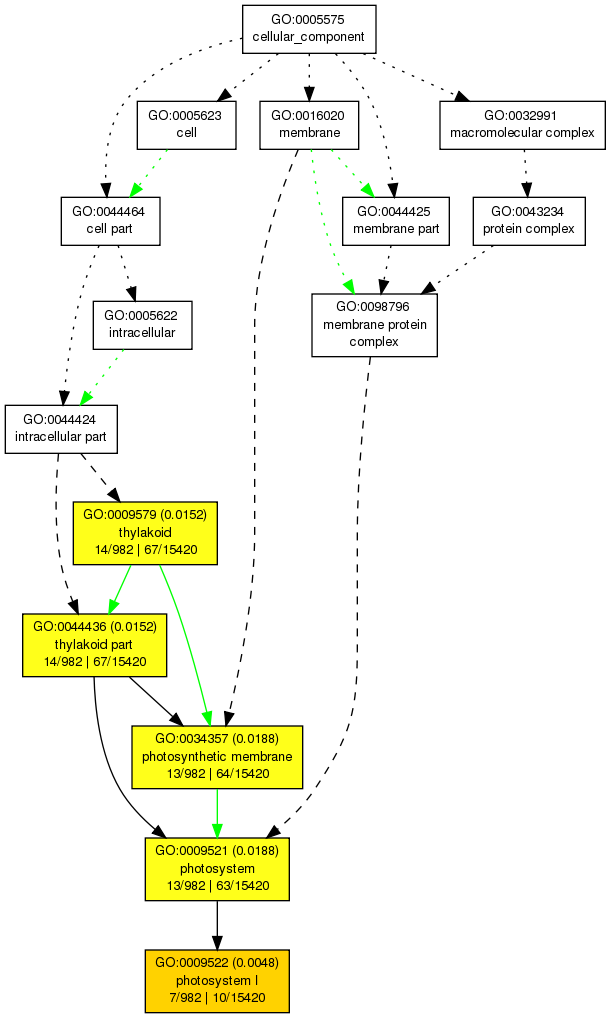
\includegraphics[width=\textwidth]{figures/agriGO_seed_wt_plasma_up_CC.png}}
    \caption{Up-regulated CC Ontology}
    \label{fig:enter-label}
\end{subfigure}
\begin{subfigure}[b]{0.48\textwidth}
    \centering
    \frame{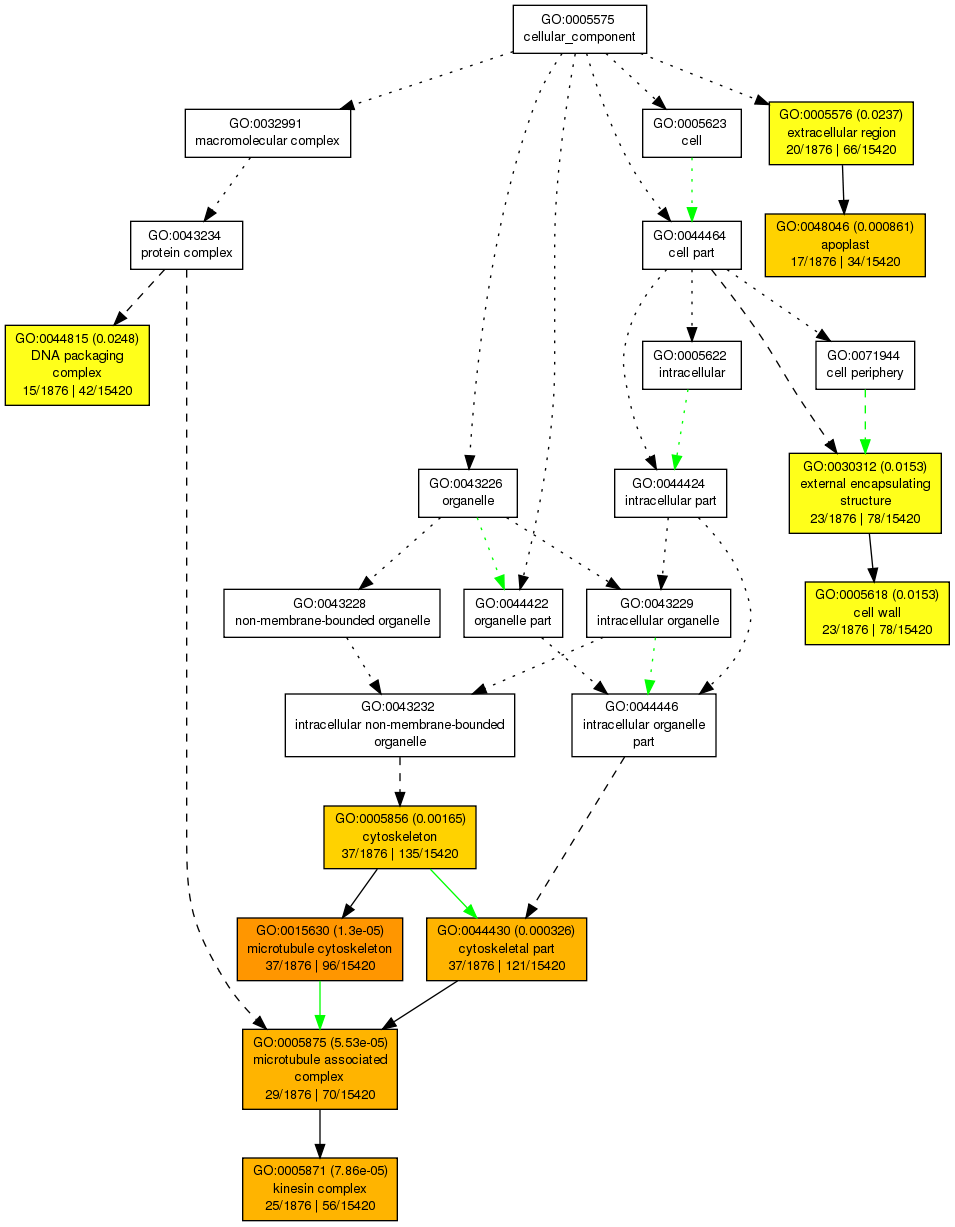
\includegraphics[width=\textwidth]{figures/agriGO_seed_wt_plasma_down_CC.png}}
    \caption{Down-regulated CC Ontology}
    \label{fig:enter-label}
\end{subfigure}
\caption{agriGO Cellular Component Ontology of (a) Up-regulated and (b) Down-regulated Genes.}
\end{figure}

Figure 7 illustrates the cellular components associated with differentially expressed genes between Seed WT and Seed Plasma conditions, as identified through agriGO analysis \parencite{tian2017agrigo}.

Subfigure (a) displays the cellular component graph of up-regulated genes, highlighting key GO terms related to photosynthetic structures and membranes. Notable terms include "photosystem I," "thylakoid," and "photosynthetic membrane," indicating the enrichment of components involved in photosynthesis and energy production in response to plasma treatment.

Conversely, Subfigure (b) presents the cellular component graph of down-regulated genes, revealing GO terms associated with cytoskeletal elements and extracellular structures. Terms such as "microtubule cytoskeleton" and "cell wall" suggest alterations in cytoskeletal organization and cell wall composition in response to plasma treatment.

\subsubsection{g:Profiler}

\begin{figure}[H]
    \centering
    \frame{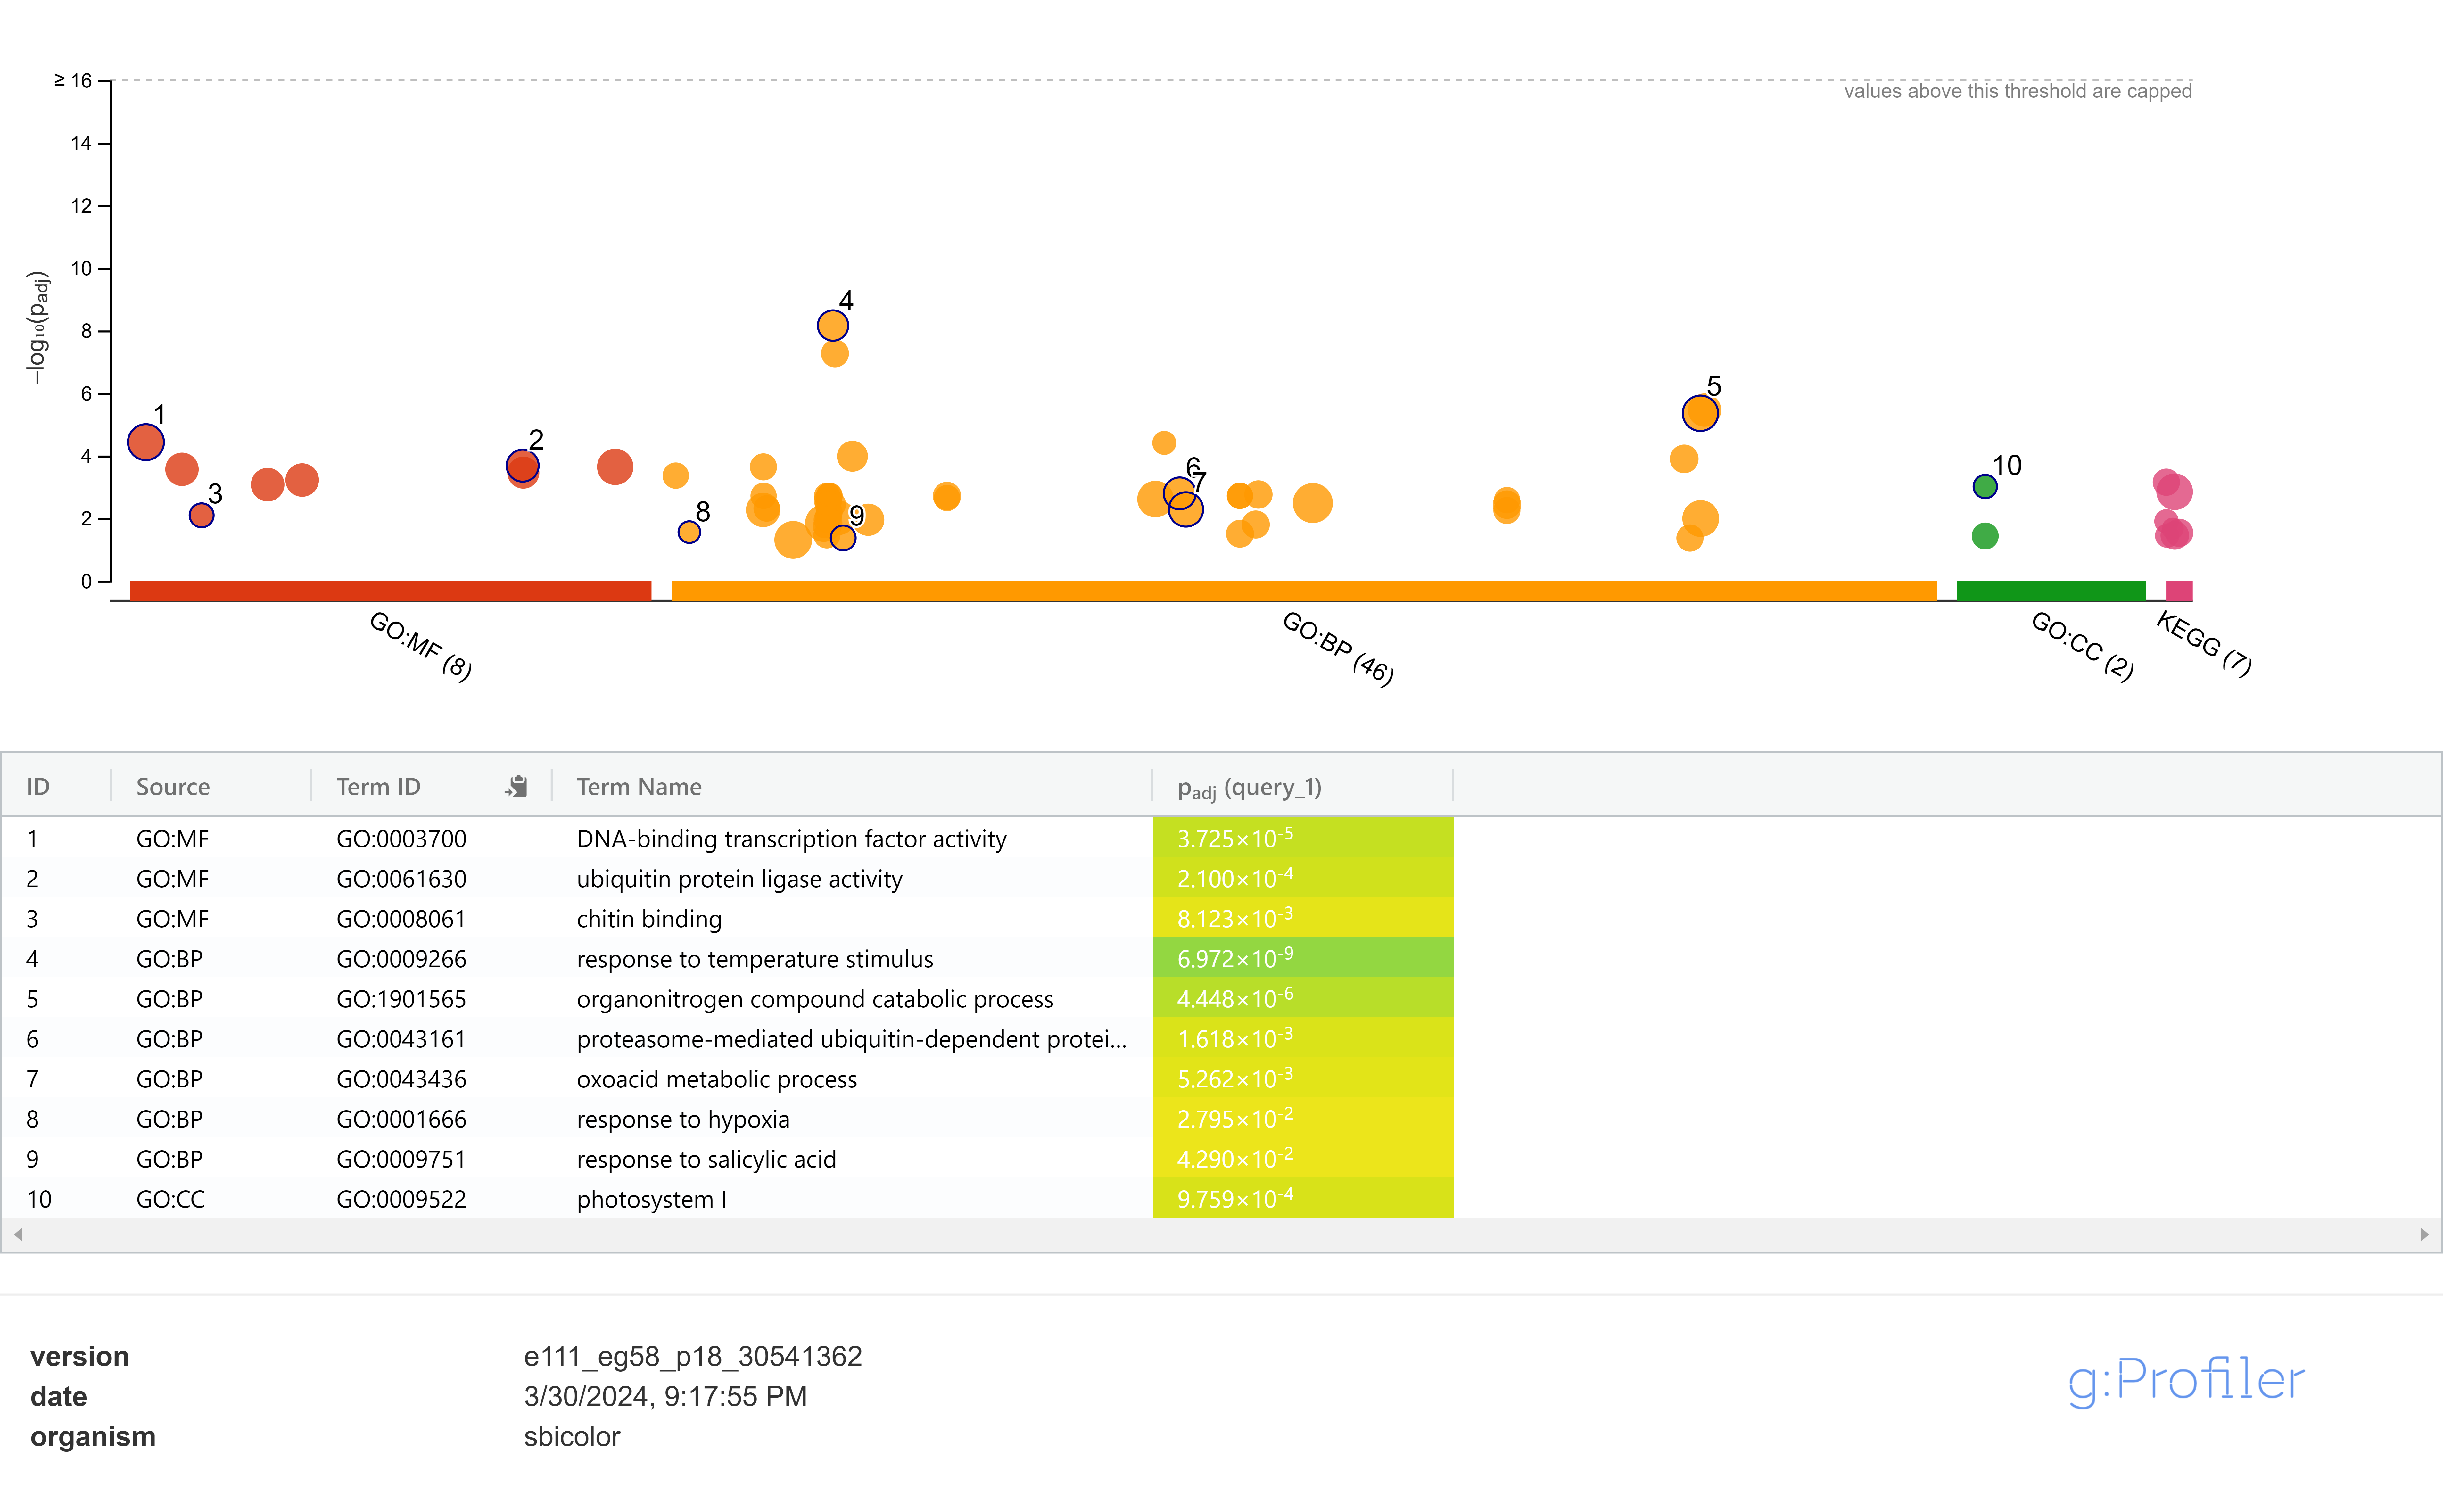
\includegraphics[width=\textwidth]{figures/gProfiler_seed_wt_plasma_up.png}}
    \caption{g:Profiler g:GOSt Result of Up-regulated Genes.}
    \label{fig:enter-label}
\end{figure}

Figure 8 presents the functional enrichment analysis results performed using the g:Profiler g:GOSt tool on the up-regulated genes between Seed WT and Seed Plasma conditions. The analysis identified several significantly enriched GO terms associated with diverse biological processes, molecular functions, and cellular components \parencite{reimand2007gProfiler}.

Among the top enriched terms, "DNA-binding transcription factor activity," "ubiquitin protein ligase activity," and "chitin binding" highlight the regulatory and protein modification functions potentially involved in response to plasma treatment. Additionally, "response to temperature stimulus" and "response to hypoxia" suggest adaptive responses to environmental cues induced by plasma treatment.

Notably, the enrichment of terms such as "proteasome-mediated ubiquitin-dependent protein" and "oxoacid metabolic process" underscores the involvement of protein degradation and metabolic processes in the cellular response to plasma treatment.

\begin{figure}[H]
    \centering
    \frame{\includegraphics[width=\textwidth]{figures/gProfiler_seed_wt_plasma_down.png}}
    \caption{g:Profiler g:GOSt Result of Down-regulated Genes.}
    \label{fig:enter-label}
\end{figure}

Figure 9 displays the functional enrichment analysis results conducted using the g:Profiler g:GOSt tool on the down-regulated genes between Seed WT and Seed Plasma conditions. The analysis identified several significantly enriched GO terms associated with various biological processes, molecular functions, and cellular components \parencite{reimand2007gProfiler}.

Among the top enriched terms, "catalytic activity," "structural constituent of chromatin," and "heme binding" highlight functional roles related to enzymatic activities and chromatin organization. Additionally, terms such as "cell wall organization or biogenesis," "mitotic cell cycle," and "secondary metabolite biosynthetic process" indicate perturbations in cellular processes and metabolic pathways associated with plasma treatment-induced gene downregulation.

Enriching terms such as "extracellular region" and "microtubule cytoskeleton" suggest cellular organization and extracellular matrix composition alterations in response to plasma treatment.

\subsubsection{PlantRegMap}

\begin{figure}[H]
\centering
\begin{subfigure}[b]{0.48\textwidth}
    \centering
    \frame{\includegraphics[width=\textwidth]{figures/PlantRegMap_seed_wt_plasma_up_ontology_BP.png}}
    \caption{Up-regulated BP Ontology}
    \label{fig:enter-label}
\end{subfigure}
\begin{subfigure}[b]{0.48\textwidth}
    \centering
    \frame{\includegraphics[width=\textwidth]{figures/PlantRegMap_seed_wt_plasma_up_histogram_BP.png}}
    \caption{Up-regulated BP Histogram}
    \label{fig:enter-label}
\end{subfigure}\par
\begin{subfigure}[b]{0.48\textwidth}
    \centering
    \frame{\includegraphics[width=\textwidth]{figures/PlantRegMap_seed_wt_plasma_up_ontology_MF.png}}
    \caption{Up-regulated MF Ontology}
    \label{fig:enter-label}
\end{subfigure}
\begin{subfigure}[b]{0.48\textwidth}
    \centering
    \frame{\includegraphics[width=\textwidth]{figures/PlantRegMap_seed_wt_plasma_up_histogram_MF.png}}
    \caption{Up-regulated MF Histogram}
    \label{fig:enter-label}
\end{subfigure}\par
\begin{subfigure}[b]{0.48\textwidth}
    \centering
    \frame{\includegraphics[width=\textwidth]{figures/PlantRegMap_seed_wt_plasma_up_ontology_CC.png}}
    \caption{Up-regulated CC Ontology}
    \label{fig:enter-label}
\end{subfigure}
\begin{subfigure}[b]{0.48\textwidth}
    \centering
    \frame{\includegraphics[width=\textwidth]{figures/PlantRegMap_seed_wt_plasma_up_histogram_CC.png}}
    \caption{Up-regulated CC Histogram}
    \label{fig:enter-label}
\end{subfigure}\
\caption{PlantRegMap Up-regulated Genes' (a) Biological Process Ontology, (b) Biological Process Histogram, (c) Molecular Function Ontology, (d) Molecular Function Histogram, (e) Cellular Component Ontology, and (f) Cellular Component Histogram.}
\end{figure}


\begin{figure}[H]
\centering
\begin{subfigure}[b]{0.48\textwidth}
    \centering
    \frame{\includegraphics[width=\textwidth]{figures/PlantRegMap_seed_wt_plasma_down_ontology_BP.png}}
    \caption{Down-regulated BP Ontology}
    \label{fig:enter-label}
\end{subfigure}
\begin{subfigure}[b]{0.48\textwidth}
    \centering
    \frame{\includegraphics[width=\textwidth]{figures/PlantRegMap_seed_wt_plasma_down_histogram_BP.png}}
    \caption{Down-regulated BP Histogram}
    \label{fig:enter-label}
\end{subfigure}\par
\begin{subfigure}[b]{0.48\textwidth}
    \centering
    \frame{\includegraphics[width=\textwidth]{figures/PlantRegMap_seed_wt_plasma_down_ontology_MF.png}}
    \caption{Down-regulated MF Ontology}
    \label{fig:enter-label}
\end{subfigure}
\begin{subfigure}[b]{0.48\textwidth}
    \centering
    \frame{\includegraphics[width=\textwidth]{figures/PlantRegMap_seed_wt_plasma_down_histogram_MF.png}}
    \caption{Down-regulated MF Histogram}
    \label{fig:enter-label}
\end{subfigure}\par
\begin{subfigure}[b]{0.48\textwidth}
    \centering
    \frame{\includegraphics[width=\textwidth]{figures/PlantRegMap_seed_wt_plasma_down_ontology_CC.png}}
    \caption{Down-regulated CC Ontology}
    \label{fig:enter-label}
\end{subfigure}
\begin{subfigure}[b]{0.48\textwidth}
    \centering
    \frame{\includegraphics[width=\textwidth]{figures/PlantRegMap_seed_wt_plasma_down_histogram_CC.png}}
    \caption{Down-regulated CC Histogram}
    \label{fig:enter-label}
\end{subfigure}\
\caption{PlantRegMap Down-regulated Genes' (a) Biological Process Ontology, (b) Biological Process Histogram, (c) Molecular Function Ontology, (d) Molecular Function Histogram, (e) Cellular Component Ontology, and (f) Cellular Component Histogram.}
\end{figure}

Figure 10 presents the functional analysis results of PlantRegMap on the up-regulated genes between Seed WT and Seed Plasma conditions. Subfigures (a), (c), and (e) depict the Biological Process Ontology, Molecular Function Ontology, and Cellular Component Ontology, respectively, highlighting the enriched GO terms associated with different aspects of gene function and localization \parencite{tian2020plantregmap}.

Notable GO terms identified in the histograms (Subfigures (b), (d), and (f)) include "response to oxygen-containing compound," "transcription factor activity," and "photosystem I," suggesting enrichment of processes related to environmental responses, transcriptional regulation, and photosynthesis in response to plasma treatment. These findings provide insights into the functional roles and cellular localization of up-regulated genes in the studied organism under plasma treatment conditions.

Similarly, Figure 11 illustrates the functional analysis results conducted using PlantRegMap on the down-regulated genes between Seed WT and Seed Plasma conditions. Subfigures (a), (c), and (e) display the Biological Process Ontology, Molecular Function Ontology, and Cellular Component Ontology, respectively, highlighting the enriched GO terms associated with various biological processes, molecular functions, and cellular components \parencite{tian2020plantregmap}.

Notable GO terms identified in the histograms (Subfigures (b), (d), and (f)) include "cell wall organization or biogenesis," "catalytic activity," and "cell wall," suggesting perturbations in processes related to cell wall organization, enzymatic activities, and cellular localization in response to plasma treatment. These findings provide insights into the functional roles and cellular localization of down-regulated genes in the studied organism under plasma treatment conditions.


\subsection{eFP Browser}


\subsubsection{TPM Correlation Analysis}
To assess the reliability of the transcript abundance estimates obtained from RNA-Seq data, a correlation analysis was performed comparing the TPM (Transcripts Per Million) values derived from the RNA-Seq experiment with the databased TPM values available in the eFP Browser’s database \parencite{wagner2012tpm}.

\begin{table}[H]
\centering
\begin{tabular}{|c|c|c|c|c|}
\hline
                        & seed\_dry\_1 & seed\_dry\_2 & seed\_dry\_3 & mean\_tpm \\ \hline
databased\_seed\_dry\_1 & 0.9053431    & 0.9104441    & 0.8561029    & 0.9101076 \\ \hline
databased\_seed\_dry\_2 & 0.8524849    & 0.8229024    & 0.7690464    & 0.8346996 \\ \hline
databased\_seed\_dry\_3 & 0.8700211    & 0.8568043    & 0.8022809    & 0.8624846 \\ \hline
databased\_mean\_tpm    & 0.8797852    & 0.8668061    & 0.8122952    & 0.8726687 \\ \hline
\end{tabular}
\caption{Correlation Coefficient Matrix of TPM and Databased TPM.}
\end{table}

The correlation analysis revealed strong positive correlations between the TPM values of samples from the RNA-Seq experiment and the databased TPM values. For instance, the correlation coefficients between samples within the RNA-Seq experiment ranged from approximately 0.77 to 0.91, indicating high consistency in transcript abundance estimates across replicates. Furthermore, the correlation coefficients between the RNA-Seq-derived TPM values and the databased TPM values ranged from approximately 0.80 to 0.91, suggesting a high degree of concordance between the two datasets.

Overall, the TPM correlation analysis underscores the reliability of the transcript abundance estimates obtained from the RNA-Seq experiment and validates the consistency of gene expression patterns observed across samples.


\subsubsection{eFP Browser Visualization}
Utilizing the Sorghum eFP Browser, gene expression patterns across different conditions were visually represented \parencite{winter2007electronic}. By searching for \textit{Sorghum bicolor} gene IDs, users can observe the gene expression levels depicted by a colour gradient ranging from red to yellow. In this representation, red signifies high gene expression levels, while yellow indicates low or negligible gene expression.

\begin{figure}[H]
    \centering
    \frame{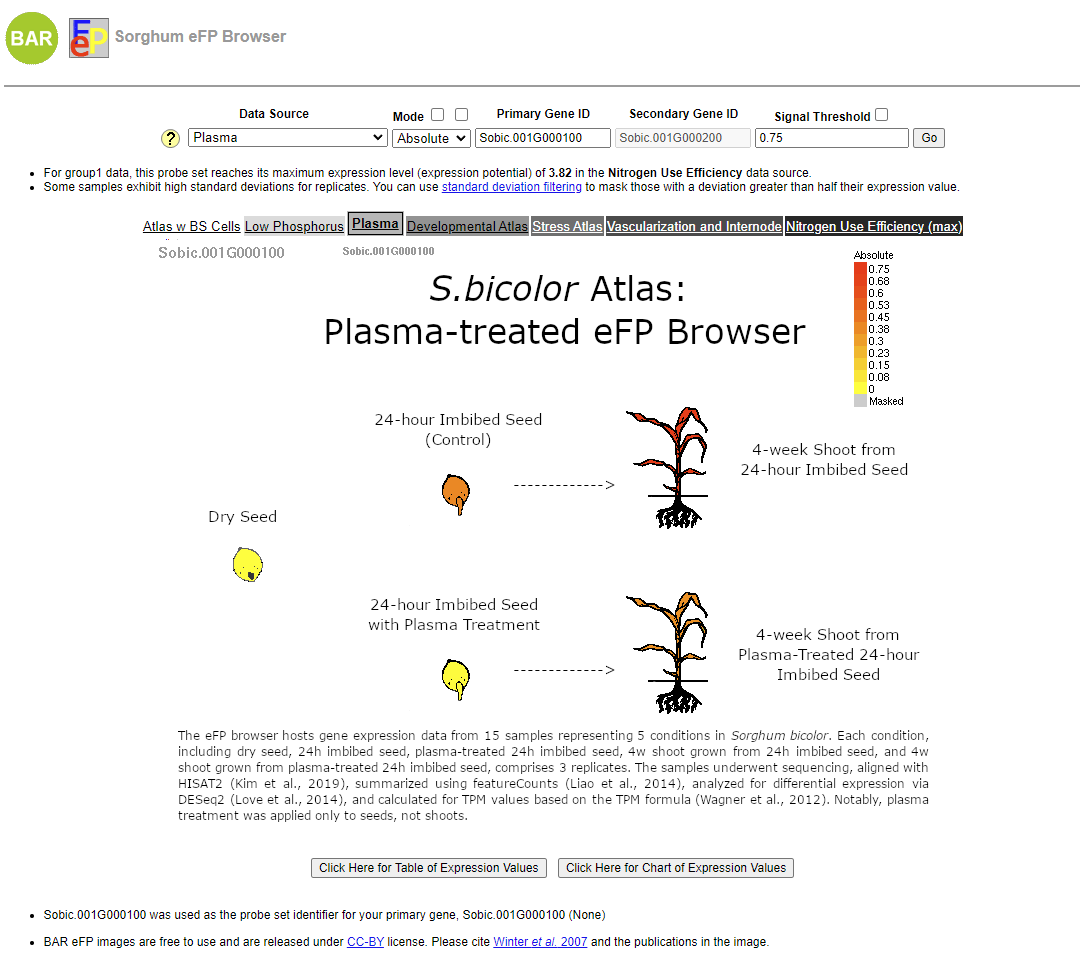
\includegraphics[width=\textwidth]{figures/eFP browser.png}}
    \caption{Sorghum eFP Browser Plasma Atlas.}
    \label{fig:enter-label}
\end{figure}

The Sorghum eFP Browser Plasma Atlas comprehensively visualizes gene expression patterns in response to plasma treatment. Through interactive exploration, users can gain insights into the spatial and temporal dynamics of gene expression changes induced by plasma treatment across the \textit{Sorghum bicolor} genome.

\section{Discussion}

The current study employed RNA-Seq analysis coupled with bioinformatics tools to explore the transcriptional response of \textit{Sorghum bicolor} to plasma treatment, revealing dynamic changes in gene expression patterns across various conditions and developmental stages.

\subsection{Differential Gene Expression Analysis}

Our analysis unveiled substantial alterations in gene expression profiles, notably identifying a significant number of up and down-regulated genes in response to plasma treatment compared to the wild-type condition. These findings offer insights into the molecular mechanisms underlying the biological effects of plasma treatment on \textit{Sorghum bicolor}.

\subsection{Functional Analysis}

Functional enrichment analysis using agriGO, g:Profiler, and PlantRegMap elucidated the biological processes, molecular functions, and cellular components associated with the differentially expressed genes. Enrichment of processes related to photosynthesis, response to environmental stimuli, and metabolic pathways underscored the multifaceted nature of the plant's response to plasma treatment. Additionally, the down-regulation of genes involved in cell wall organization and carbohydrate metabolism suggests the potential remodelling of cell structure and metabolism in response to plasma treatment.

\subsection{eFP Browser}

Using the Sorghum eFP Browser, visualizing gene expression patterns provided valuable insights into the spatial and temporal dynamics of gene expression changes induced by plasma treatment. Observing gene expression levels in different tissues and developmental stages enhances our understanding of the systemic response of \textit{Sorghum bicolor} to plasma treatment.

\subsection{Implications and Future Directions}

These findings contribute to understanding the molecular mechanisms underlying \textit{Sorghum bicolor}'s response to plasma treatment. Insights gained could improve crop resilience and productivity under various environmental conditions. Future research may focus on elucidating specific regulatory networks and signalling pathways involved in response to plasma treatment, as well as exploring applications in agricultural practices to enhance crop growth and stress tolerance.

\subsection{Limitations}

Acknowledging the limitations of this study is crucial. While RNA-Seq analysis provides valuable insights into gene expression patterns, further experimental validation is necessary to confirm the functional significance of identified differentially expressed genes. Additionally, our analysis focused on specific conditions and developmental stages, warranting further studies encompassing a broader range of conditions and time points for a comprehensive understanding of the transcriptional response to plasma treatment in \textit{Sorghum bicolor}.

\subsection{Conclusion}

In conclusion, our study sheds light on the transcriptional response of \textit{Sorghum bicolor} to plasma treatment, revealing dynamic changes in gene expression patterns. The comprehensive analysis provided valuable insights into the molecular mechanisms underlying the response to plasma treatment, offering potential implications for agricultural practices and crop improvement strategies.

\clearpage
\nocite{*}
\printbibliography

\end{document}

